\chapter{Introdução}

    Os métodos comumente utilizados de sensoriamento do coração podem ser separados em três classes, a detecção de sinais elétrico gerados pelo sistema cardíaco, geralmente feita por ECG, a detecção das movimentações mecânicas do sistema cardíaco, geralmente feita por fonocardiograma, e a observação do coração por métodos de visualização, geralmente feito por ecocardiograma. Embora a terceira classe tenha uma capacidade de diagnostico superior as outras ela exige um ambiente controlado e geralmente um maquinário grande e de alto custo, e portanto não será foco desse estudo.

    A detecção de sinais elétricos cardíacos por meio do eletrocardiograma (ECG)  é usualmente o método padrão de sensoriamento contínuo utilizado, uma vez que o sinal elétrico cardíaco tem relativamente pouca variação, mesmo comparando o sinal de diferentes pacientes, e já foi amplamente estudado, tornando sua análise simples e sua detecção bem padronizada e de fácil implementação, tornando detecção de eventos simples, como batimentos por minuto (bpm), fácil e confiável. O problema da detecção do sinal elétrico é que esse é o ativador das etapas do ciclo cardíaco, portanto não temos informação direta sobre o movimento real do coração, somente a influência que esse tem sobre o sinal elétrico seguinte.

    Por outro lado, a detecção dos sinais mecânicos do sistema cardíaco é realizada, quase exclusivamente, por fonocardiograma (PCG), que é a detecção do som produzido pelo ciclo cardíaco, e geralmente de forma não automatizada, ou seja é geralmente realizada pelo médico utilizando um estetoscópio e seu conhecimento para detectar e analisar o sinal. Essa técnica permite ao médico uma análise qualitativa do estado atual do coração do paciente, mas, por ser uma técnica dependente da audição do médico, não permite uma análise quantitativa, além de depender da capacidade do médico que esta realizando a técnica.%Preciso checar se isso é verdade e pegar umas fontes
Diversas tentativas de automatizar esse processo estão sendo feitas, mas ainda não estão sendo utilizadas na prática. %Preciso de referências e razão da dificuldade 

    Outros dois métodos de sensoriamento mecânico do ciclo cardíaco que estão ganhado espaço e atenção nas pesquisas teóricas da área são o balistocardiograma (BCG) e o seismeocaridograma (SCG). Esses dois métodos foram continuamente estudados durante o século 20, mas devido a problemas tecnológicos e ao avanço de outros tipos de medições foram deixados de lado, e somente agora estão ganhando novamente seu espaço entre os métodos de sensoriamento \cite{ballistoAndSeisReview}.
    
    O balistocardiograma tem como objetivo observar as vibrações no corpo geradas pela ejecção de sangue do sistema cardíaco, geralmente realizado por meio de uma balança, uma cadeira ou uma cama com sensoriamento. Como o sinal a ser observado é geralmente de uma ordem de grandeza bem menor do que o peso do paciente, sua detecção se torna complicada e a extração de dados do sinais geralmente se torna restrita \cite{ballistoAndSeisReview}, O sinal padrão desse método pode ser visto na figura \ref{fig:sigs}. 
%FIGURA DOS SINAIS PADRÕES DA ballistoAndSeisReview    
%Talvez falar algo como "pode ser usado para a detecção de batimentos cardíacos durante o sono e etc...

\begin{figure}[H]
    \center
    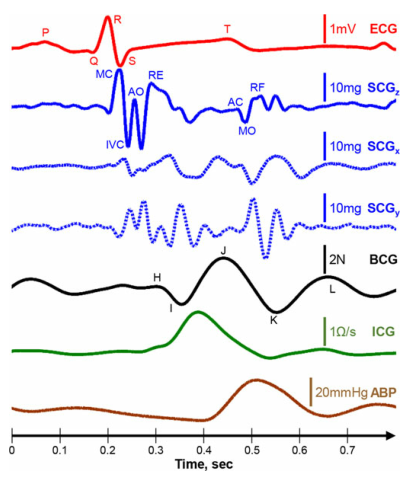
\includegraphics[width=0.4\linewidth]{img/sisBalRevFig1.png}
    \caption{Exemplo de sinal para acelerômetro triaxial, balistocardiogram, eletrocardiograma entre outros}
    \label{fig:sigs}
\end{figure}

    O seismeocardiograma utiliza um medidor de vibrações, geralmente colocado na região torácica, para detectar as movimentações da caixa torácica em resposta aos batimentos cardíacos\cite{ballistoAndSeisReview}. Uma vez que a medição é feita diretamente na região torácica, ela é independente do peso do paciente, mas é fortemente afetada pela inércia do sistema de detecção e por qualquer outro movimento realizado pelo paciente. Considerando os grandes avanços em sensores de acelerômetros realizados nos últimos anos 
%Seria bom ter uma referência e uns dados tipo precisão e massa atual
e dos microcontroladores somos capazes de criar sistemas de medição com grande precisão e pequena inercia que conseguem continuamente ler, armazenar, transmitir e analisar o sinal de aceleração da caixa torácica\cite{06347128}. Como consequência as pesquisas nesse método cresceram, focando inicialmente na detecção de batimento cardíaco contínuo e na padronização dos métodos de medição\cite{06567772}.

     Grande parte das pesquisas atuais tem o foco nas vibrações com direção dorso-ventral, uma vez que essa geralmente trás mais informações relevantes, mas, com o aumento do uso de acelerômetros de três eixos, o estudo paralelo de todos os eixos é possível \cite{3dPrecordialAccSignal}, uma imagem padrão desse sinal pode ser visto na figura: %FIGURA DOS SINAIS PADRÕES DA ballistoAndSeisReview
Um dos grandes problemas desse método, é que, diferente do ECG, seu sinal sofre grandes variações, mesmo quando medidos de um mesmo paciente\cite{3dPrecordialAccSignal}\cite{heartbeatSegInSeismocardiograms}\cite{06945019}, tornando detecções simples, como batimento cardíaco, difíceis e não confiáveis. Um exemplo do sinal de 5 batimentos de dois pacientes, um saudável e outro com isquemia podem ser vistos na figura \ref{fig:5bat}. %Talvez falar um pouco de alguns resultados e do uso de 3d e giroscópio

\begin{figure}[H]
    \center
    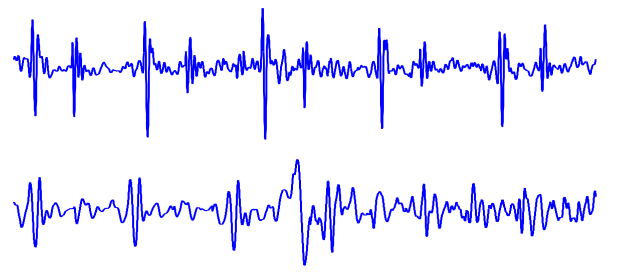
\includegraphics[width=0.4\linewidth]{img/06945019_1.png}
    \caption{sinal do sismeocardiograma de 2 pacientes, durante 5 batimentos cardíacos, o gráfico superior é de um paciente saudável, e o inferior é de um paciente diagnosticado com isquemia}
    \label{fig:5bat}
\end{figure}


    Embora essa dificuldade o sismeocardiograma se apresenta como uma possível alternativa de baixo custo para a análise e monitoramento contínuo e não invasivo da qualidade do ciclo cardíaco do paciente\cite{06611240}, dado que se encontrem caminhos robustos para se interpretarem seus dados sem a necessidade de supervisão humana ou grande quantidade de recursos computacionais

    Um ponto importante a se observar sobre esse três últimos métodos é que todos eles observam o resultado dos movimentos do coração, na sua forma física, tornando possível uma análise do real funcionamento cardíaco, independente do sistema nervoso. Isso poderia levar a possíveis sistemas de diagnósticos poderosos e portáteis, mas somente se algum método de análise for desenvolvido que seja capaz de obter dados significantes e de maneira confiável. 
